\documentclass[]{scrartcl}
\usepackage[utf8]{inputenc}
\usepackage{amsthm}
\usepackage{amssymb}
\usepackage{amsmath}
\usepackage{calc}
\usepackage{graphicx}
\usepackage[ngerman, german]{babel}
\usepackage{caption}
\usepackage{array}

\makeatletter
\newcommand{\thickhline}{%
    \noalign {\ifnum 0=`}\fi \hrule height 1pt
    \futurelet \reserved@a \@xhline
}
\makeatother


\newcommand{\R}{\mathbb{R}}
\newcommand{\N}{\mathbb{N}}

\title{Modulbegleitende Aufgabe II}
\author{Shanshan Huang, Florian Starke}
\begin{document}
	\maketitle
	Gegeben seien $N\in\N$, eine Zerlegung $\Delta_N$ des Intervalls $[-1,1]$ durch die Stützstellen $-1\leq x_0\leq x_1\leq\dots\leq x_N\leq1$, und die Funktionen $f_R,f_1\colon\R\to\R$ mit
	\[f_R(x):=\frac{1}{1+25x^2},\]
	\[f_1(x):=(1+\cos(\frac{3}{2}\pi x))^{2/3}.\]
	\section{Polynominterpolation}
	\subsection{Gleichverteilte Stützstellen}
	Die $N+1$ Stützstellen sind äquidistant verteilt. Es folgt $x_i:=-1+2i/N$ für $i=0,\dots,N$.
	\begin{figure}[h]
		\centering
		\begin{minipage}{0.5\textwidth}
			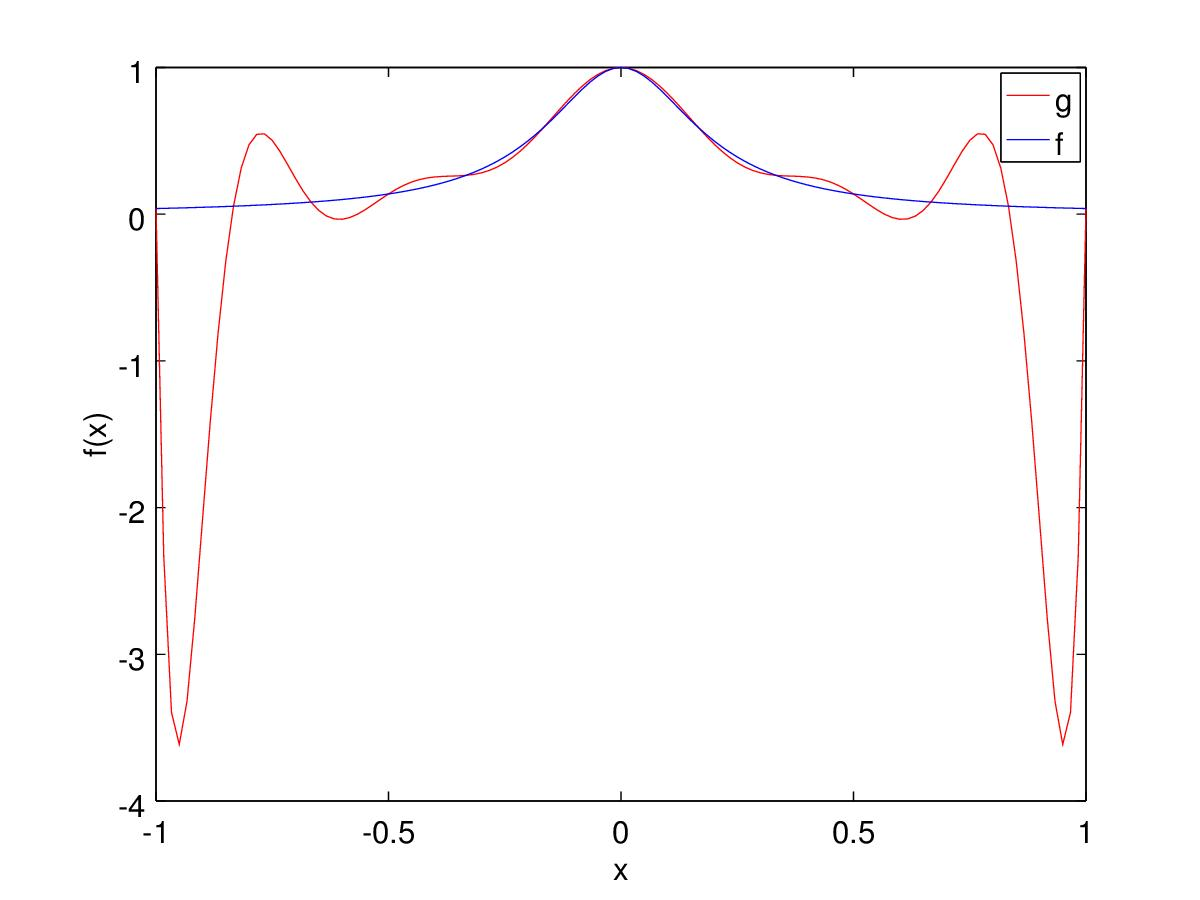
\includegraphics[width=8cm,keepaspectratio]{runge_aequidistant}
			\caption{\label{Abb.1}}
		\end{minipage}
		\begin{minipage}{0.49\textwidth}
			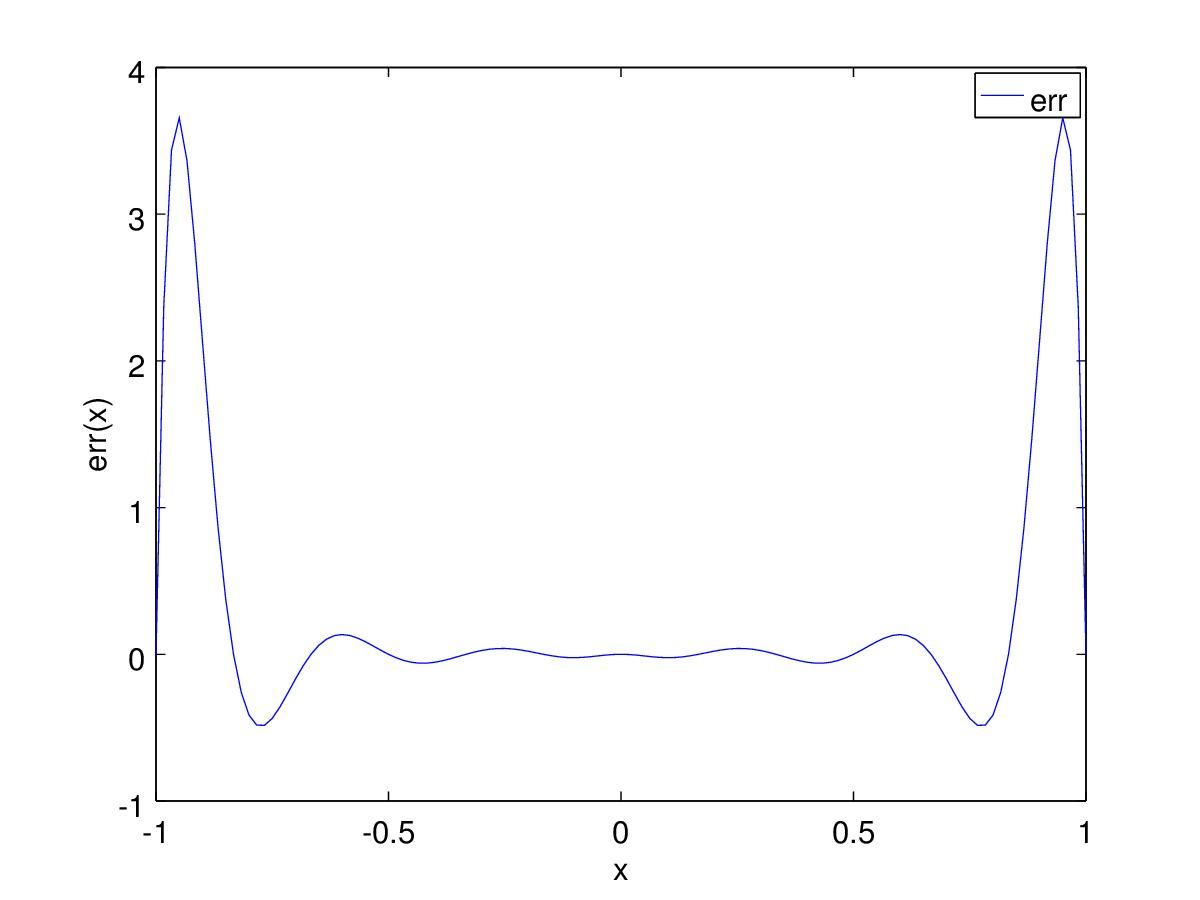
\includegraphics[width=8cm,keepaspectratio]{runge_err}
			\caption{\label{Abb.2}}
		\end{minipage}
	\end{figure}
	
	In Abbildung \ref{Abb.1} ist $f_R$ und das interpolierte Polynom $g_{12}$ abgebildet. Wie erwartet ist bei einer Gleichverteilung der Stützstellen ....
	\subsection{Tschebyschow-Stützstellen}
	Als Stützstellen werden die Nullstellen des Tschebyschow-Polynoms $T_{N+1}$ gewählt. Also definieren wir $x_i:=\cos(\frac{2k-1}{2N+2}\pi)$ für $i=0,\dots,N$.
	
	\begin{figure}[h]
		\centering
		\begin{minipage}{0.5\textwidth}
			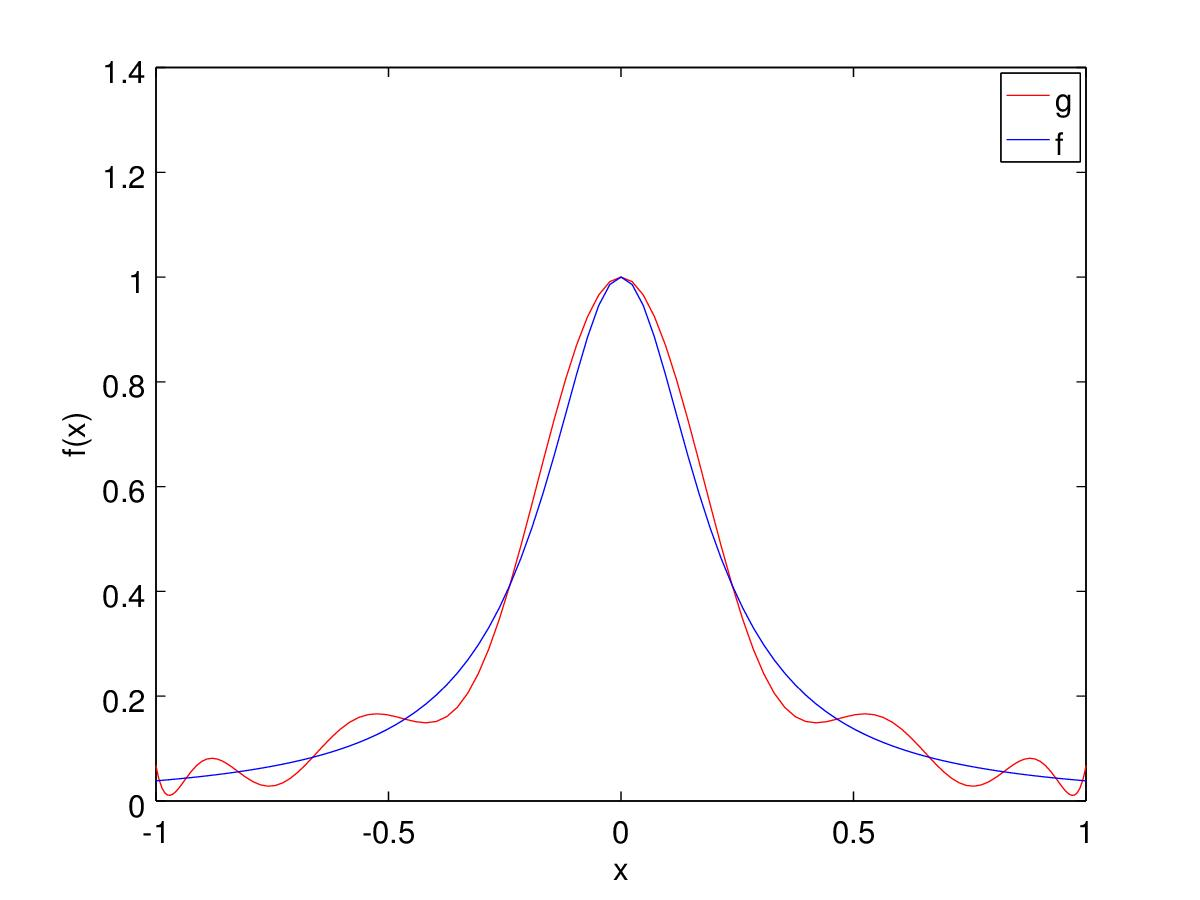
\includegraphics[width=8cm,keepaspectratio]{runge_tscheb}
			\caption{\label{Abb.3}}
		\end{minipage}
		\begin{minipage}{0.49\textwidth}
			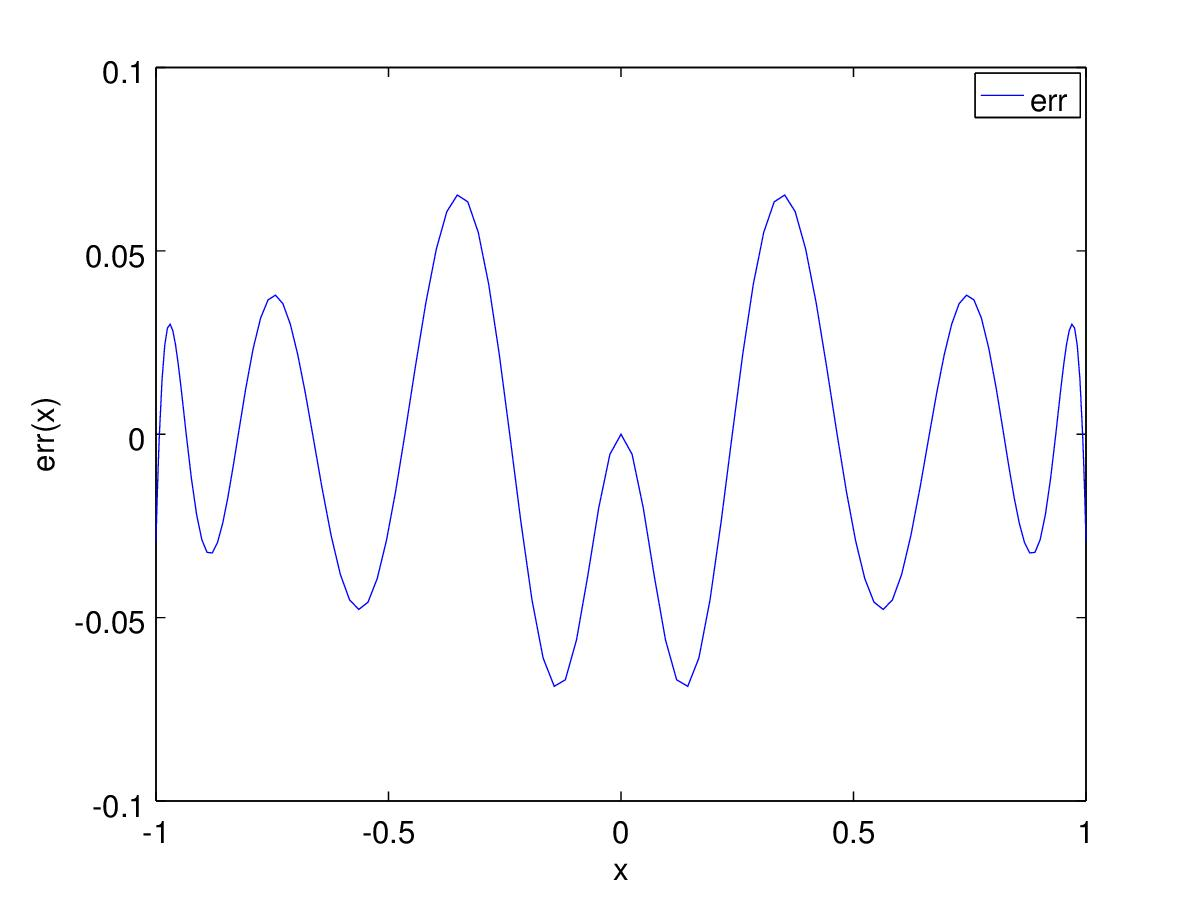
\includegraphics[width=8cm,keepaspectratio]{runge_tscheb_err}
			\caption{\label{Abb.4}}
		\end{minipage}
	\end{figure}
	
	\section{Spline-Interpolation}
	\begin{figure}[h]
		\centering
		\begin{minipage}{0.5\textwidth}
			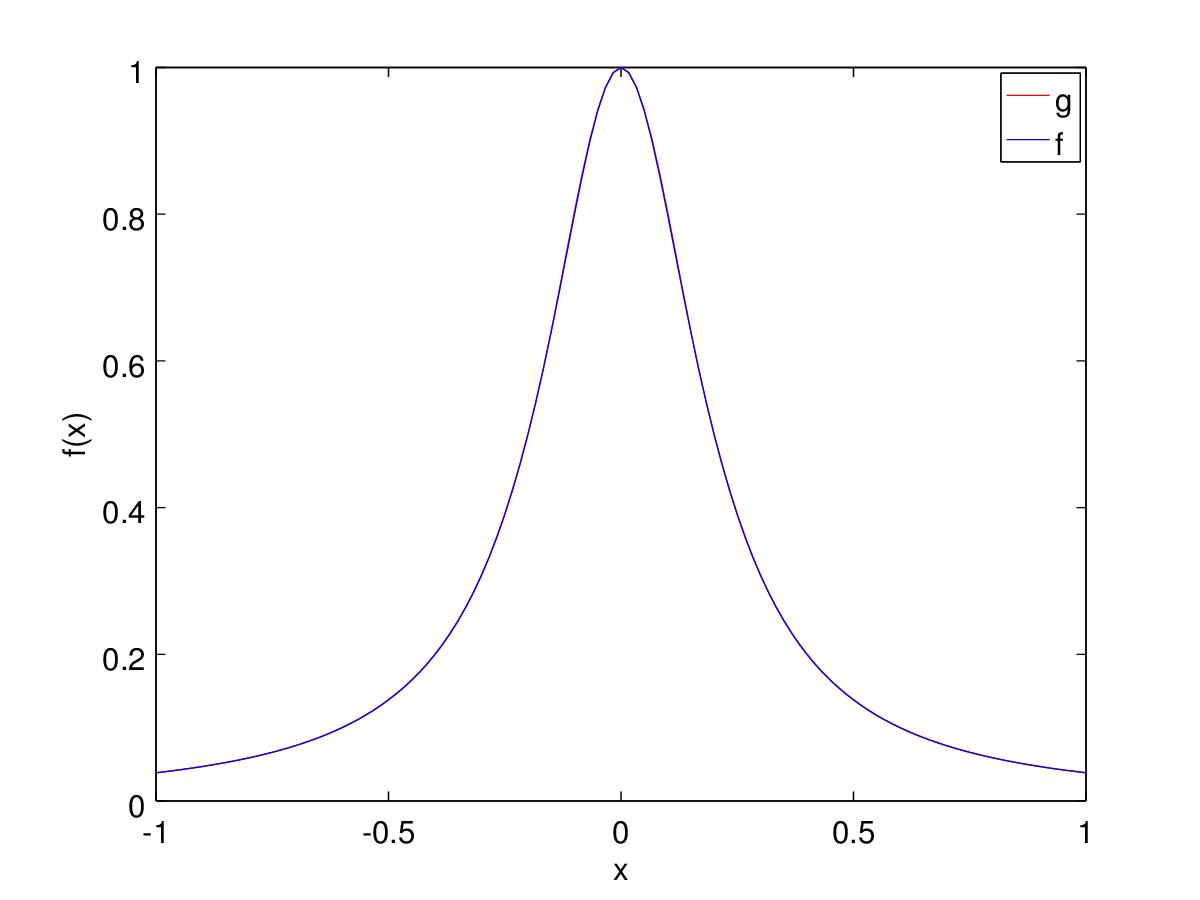
\includegraphics[width=8cm,keepaspectratio]{runge_spline}
			\caption{\label{Abb.5}}
		\end{minipage}
		\begin{minipage}{0.49\textwidth}
			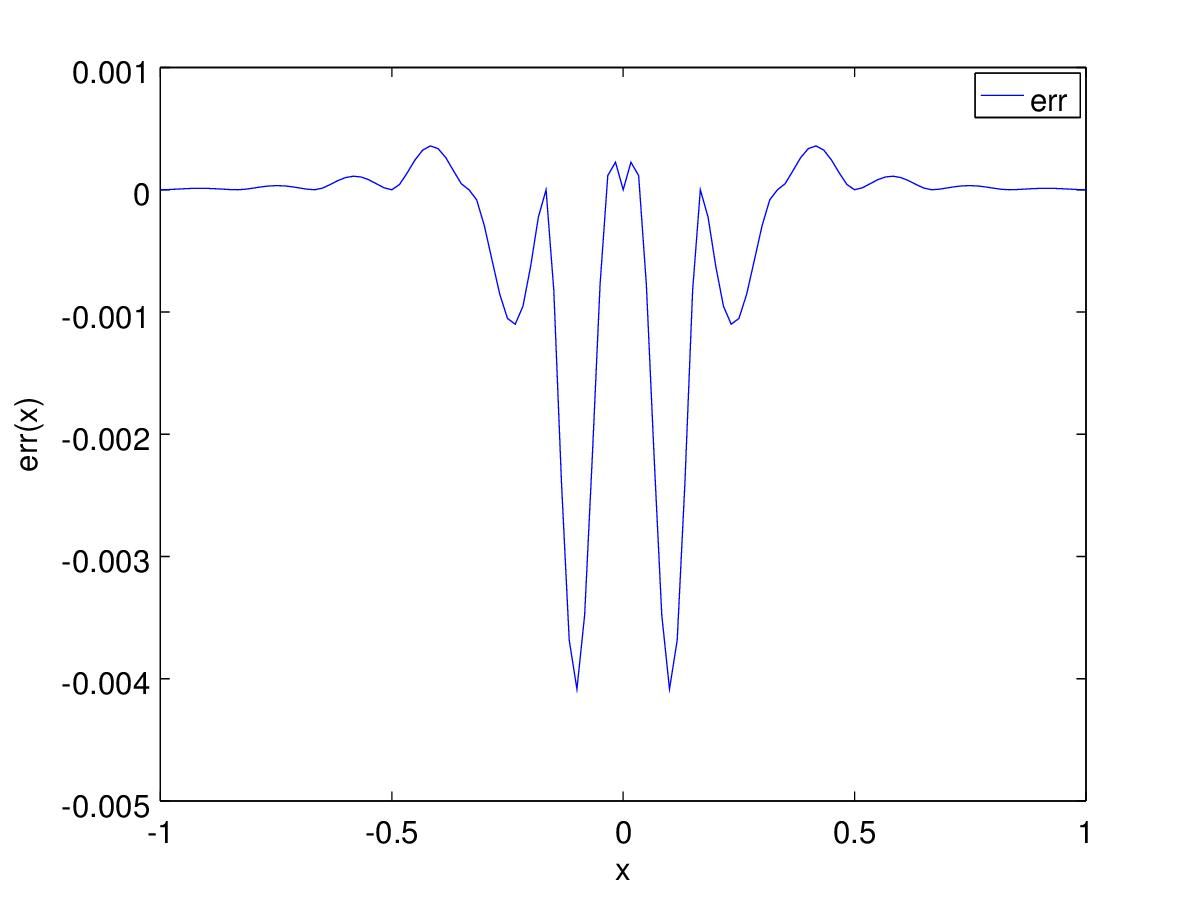
\includegraphics[width=8cm,keepaspectratio]{runge_spline_err}
			\caption{\label{Abb.6}}
		\end{minipage}
	\end{figure}
	
	Fehler für $N_1=2$, $N_2=4$, und $N_3=8$.
	 \begin{figure}[h]
 		\centering
 		\begin{minipage}{0.5\textwidth}
 			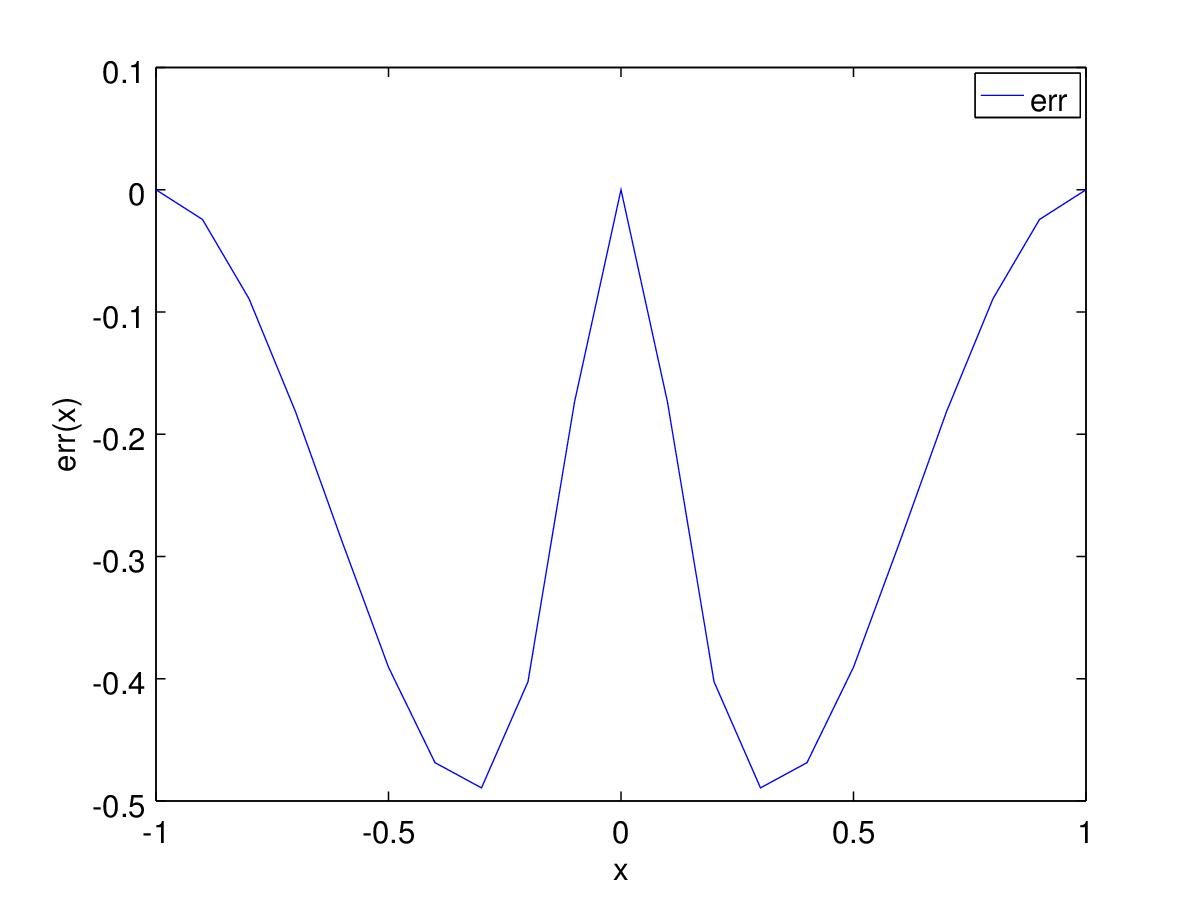
\includegraphics[width=8cm,keepaspectratio]{runge_spline_err_1}
 			\caption{$N_1$\label{Abb.7}}
 		\end{minipage}
 		\begin{minipage}{0.49\textwidth}
 			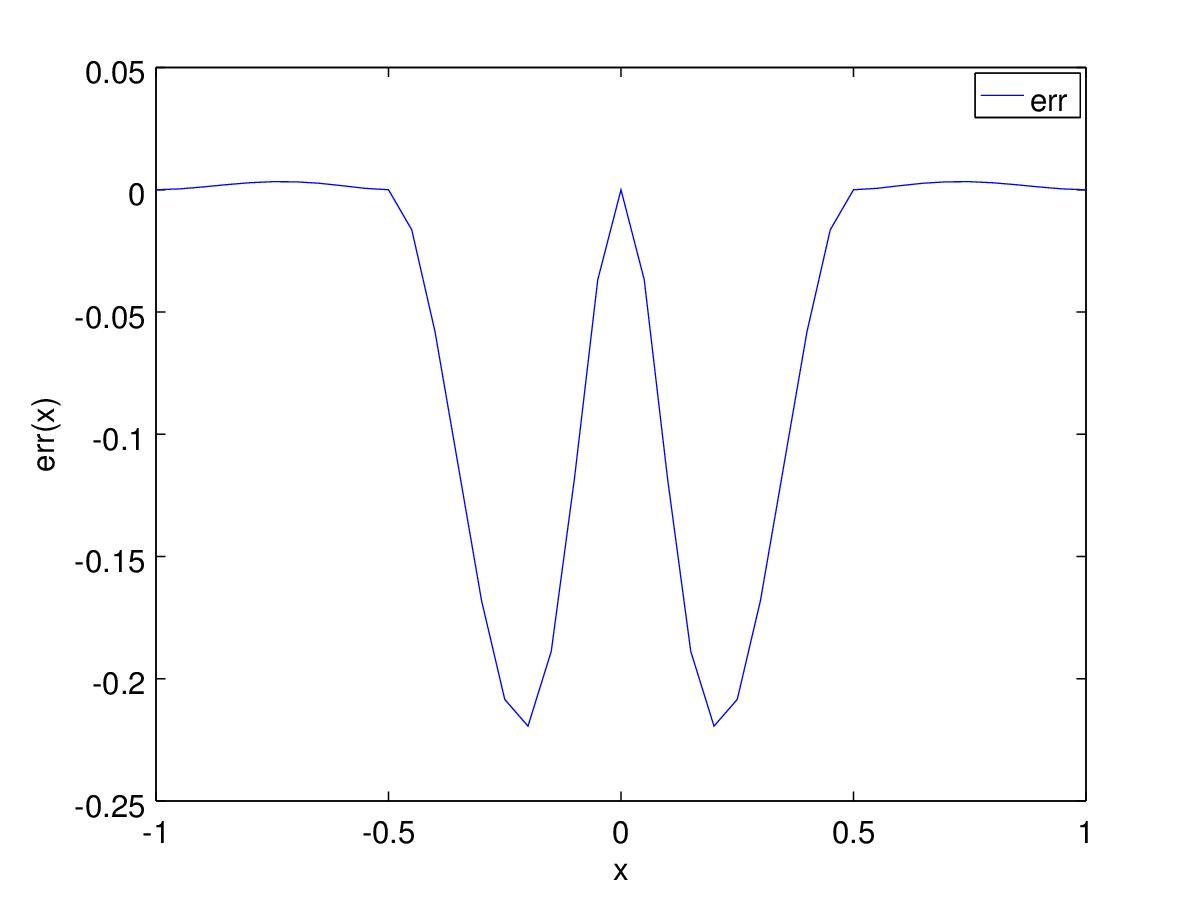
\includegraphics[width=8cm,keepaspectratio]{runge_spline_err_2}
 			\caption{$N_2$\label{Abb.8}}
 		\end{minipage}
 	\end{figure}
 	
 	\begin{figure}[h]
 		\centering
		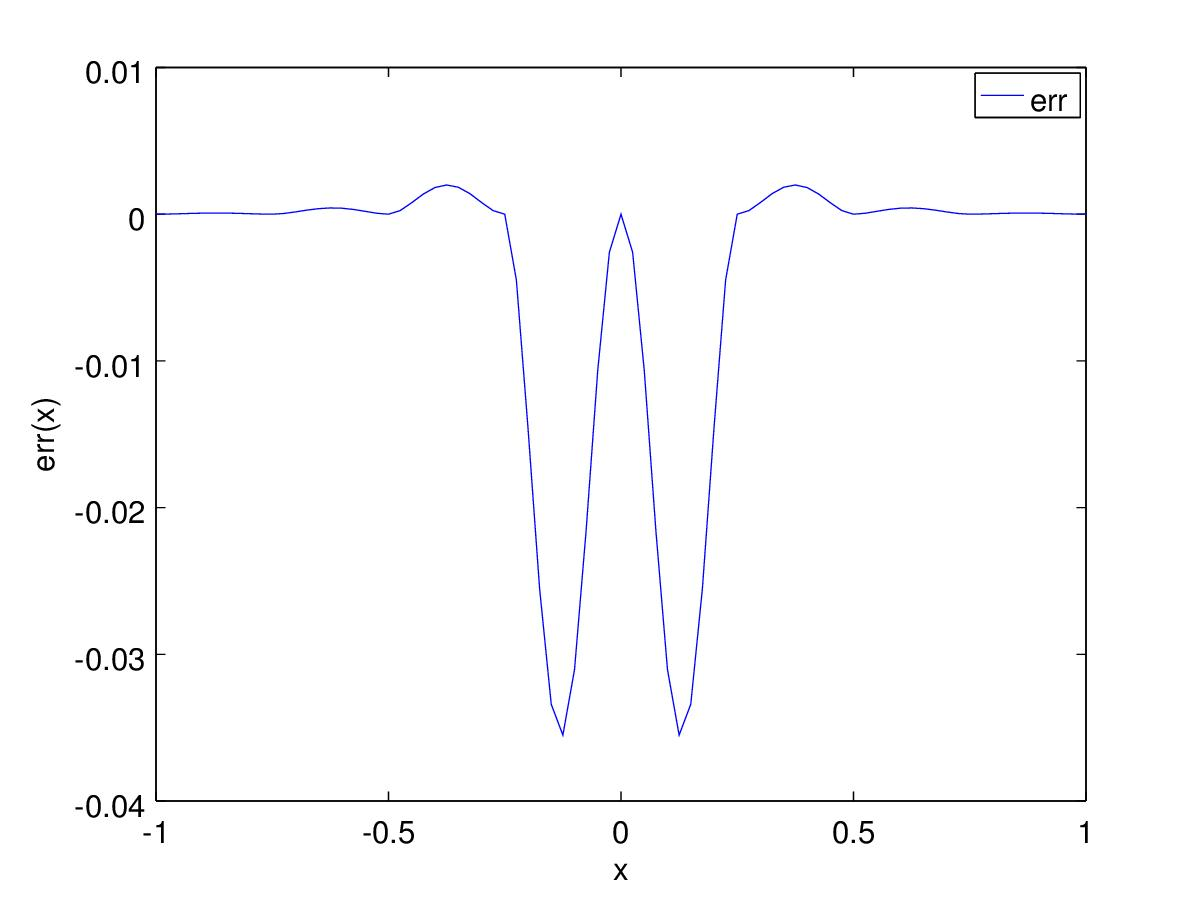
\includegraphics[width=8cm,keepaspectratio]{runge_spline_err_3}
		\caption{$N_3$\label{Abb.9}}
 	\end{figure}
 	
 	\renewcommand{\arraystretch}{1.2}
 	\begin{tabular}{|c|c|c|}\hline
 	$k$  & $E(h_{N_k})$ & $\operatorname{EOC}(h_{N_k},h_{N_{k+1}})$\\\thickhline
 	$1$  & $4.8928\times10^{-1}$ & $1.1572$\\\hline
 	$2$  & $2.1938\times10^{-1}$ & $2.6272$\\\hline
 	$3$  & $3.5509\times10^{-2}$ & $4.3901$\\\hline
 	$4$  & $1.6935\times10^{-3}$ & $2.1237$\\\hline
 	$5$  & $3.8860\times10^{-4}$ & $3.5334$\\\hline
 	$6$  & $3.3560\times10^{-5}$ & $3.8869$\\\hline
 	$7$  & $2.2686\times10^{-6}$ & $3.9719$\\\hline
 	$8$  & $1.4917\times10^{-7}$ & $3.9930$\\\hline
 	$9$  & $9.0802\times10^{-9}$ & $3.9982$\\\hline
 	$10$ & $5.6820\times10^{-10}$ & $3.9996$\\\hline
 	$11$ & $3.5523\times10^{-11}$ & $3.9999$\\\hline
 	$12$ & $2.2204\times10^{-12}$ & $-$\\\hline
 	\end{tabular} 
\end{document}
